\section*{Bài 2.}

Viết chuong trình giải phương trình bậc 2.
	
\addcontentsline{toc}{section}{Bài 2}

\centering
\textbf{\underline{Bài làm:}}

\justifying
\textbf{Mã giả của thuật toán:}
\begin{algorithm}
\setstretch{1.15}
\renewcommand{\algorithmcfname}{Thuật toán}

\caption{Thuật toán giải phương trình bậc 2}
\SetKwInOut{Input}{Đầu vào}\SetKwInOut{Output}{Đầu ra}
\SetAlgoNoEnd\SetAlgoNoLine%

\Input{Các số thực $a$, $b$, $c$ ($a \neq 0$).}
\Output{Các số $x$ thỏa mãn $ax^2 + bx + c = 0$.}
$d \gets b^2 - 4ac$\\
\uIf{$d > 0$}{
    $x_1 \gets \displaystyle \frac{-b + \sqrt{d}}{2a}$, $x_2 \gets \displaystyle \frac{-b - \sqrt{d}}{2a}$\\
    \Return $x_1, x_2$
}\uElseIf{$d = 0$}{
    $x_1 \gets \displaystyle \frac{-b}{2a}$\\
    $x_2 \gets x_1$\\
    \Return $x_1, x_2$
}\Else{
    \Return "Phương trình vô nghiệm"
}
\end{algorithm}


\textbf{Hiện thực thuật toán trên Maple:}

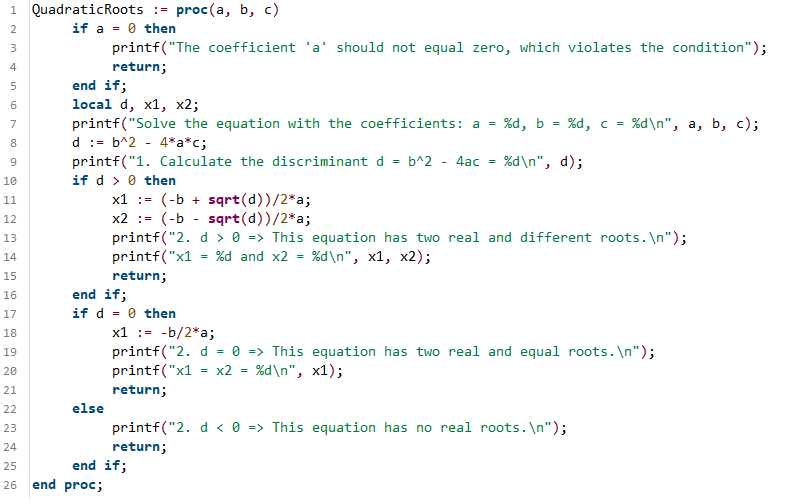
\includegraphics[width=1.0\textwidth]{images/bai2_quadraticroots.png}

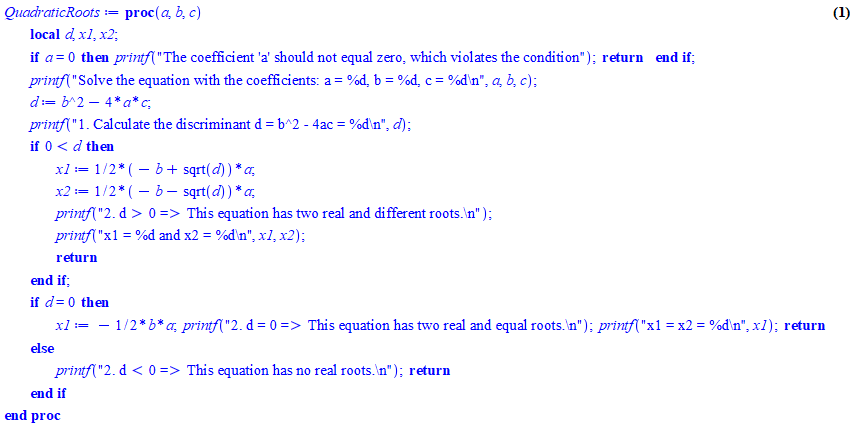
\includegraphics[width=1.0\textwidth]{images/bai2_quadraticroots_1.png}
\\[9pt]
\textbf{Một số kết quả thể hiện các bước giải phương trình bậc hai:}

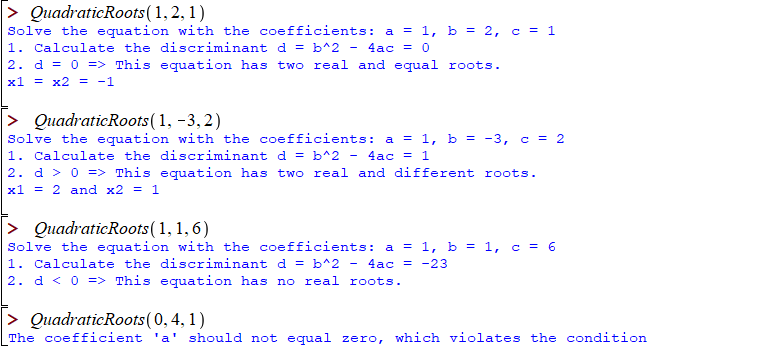
\includegraphics[width=1.0\textwidth]{images/bai2_quadraticroots_2.png}
	
\clearpage